%
% File acl2014.tex
%
% Contact: koller@ling.uni-potsdam.de, yusuke@nii.ac.jp
%%
%% Based on the style files for ACL-2013, which were, in turn,
%% Based on the style files for ACL-2012, which were, in turn,
%% based on the style files for ACL-2011, which were, in turn,
%% based on the style files for ACL-2010, which were, in turn,
%% based on the style files for ACL-IJCNLP-2009, which were, in turn,
%% based on the style files for EACL-2009 and IJCNLP-2008...

%% Based on the style files for EACL 2006 by
%%e.agirre@ehu.es or Sergi.Balari@uab.es
%% and that of ACL 08 by Joakim Nivre and Noah Smith

\documentclass[11pt]{article}
\usepackage{acl2014}
\usepackage{times}
\usepackage{url}
\usepackage{latexsym}
\usepackage{hyperref}

\usepackage{multirow}
\usepackage{tikz}
\usetikzlibrary{shapes.geometric, arrows}

\usepackage{tabularx}

%\setlength\titlebox{5cm}

% You can expand the titlebox if you need extra space
% to show all the authors. Please do not make the titlebox
% smaller than 5cm (the original size); we will check this
% in the camera-ready version and ask you to change it back.


\title{Solving Algebraic Word Problems with Semantic Parsing}

\author{John Newcomb \\
  Stanford University \\
  {\tt jnewcs@stanford.edu} \\\And
  Sloane Sturzenegger \\
  Stanford University \\
  {\tt sloanes@stanford.edu} \\}

\date{}

\begin{document}
\maketitle
\begin{abstract}
Algebraic word problems are a fundamental part of the modern math educational system. These questions test students' abilities to translate a paragraph of text into practical equations and then solve those equations using standard algebra techniques. In this paper, we introduce a semantic parsing system to extract the fundamental representation of a word problem as a system of equations. We leverage existing computer algebra systems to solve for a final result for each question. Our research confirms the findings of other literature addressing this problem; semantic parsing systems do result in high-accuracy solutions to word problems but the high number of handwritten rules required limits the amount of word problems the systems can solve at all.
\end{abstract}

\section{Introduction}
The goal of this project is to solve word problems of the type that occur on standardized tests. Mainly, we are interested in simple algebra-based problems like the following example. While our initial goal was to solve SAT-like questions that are at the upper high-school level, our survey of the current state of the art and available datasets indicated that solving SAT-level problems is beyond the scope of a one-quarter project. The example below highlights the type of word problem our system will focus on \cite{Shi:15}.

\textit{Three times the sum of three consecutive integers x, x + 1, and x + 2, is 72. What are the integers?}

\underline{Solution:}
\begin{center}
    \small{\texttt{
        3 * ( x + (x + 1) + (x + 2) ) = 72\\
        (3x + 3) = 24\\
        3x = 21\\
        (x = 7), (x+1 = 8), (x+2 = 9)
    }}
\end{center}

Questions like the one above are interesting because they can represent any complicated equation of multiple variables. A fairly complicated understanding of the sentence's semantics is necessary. For example, in the question above we need to realize that we have to not only determine that x = 7, but also return the quantities for x+1 and x+2. We believe that the learnings and intuitions from this project can be combined with more sophisticated NLP techniques to solve general higher-level word problems where the fundamental equations are similar but the amount of text and extraneous information is much higher.

The challenges of developing a computer program to solve word problems represents a fundamental dichotomy in terms of what automated systems can solve easily and what they cannot. Even the most basic computer can solve equations of one variable (like 3x = 21) much faster and with infinitely more accuracy than an eighth grader. However, a young human still outperforms advanced NLP computer systems when drawing conclusions and reasoning about textual data. The authors of Microsoft's SigmaDolphin research project (which is the research most similar to ours) argue that the reason for this difference ``lies in our amazing power of natural language understanding and reasoning (especially common sense reasoning) over state-of-the-art artificial intelligent (AI) systems.''\footnote{Microsoft Research: http://research.microsoft.com/en-us/projects/dolphin/}

Our research demonstrates this contrast particularly well. While our system solves the algebraic equations perfectly every time, it can only understand questions that are parsed by our grammar rules (which are, for the most part, written by hand). If our program cannot parse a question and form a semantic representation, we cannot solve it. Our semantic parsing system handles test-set questions that are similar to the development set very well, but fails on any type of question that is fundamentally different from any training sentence. When evaluated on our test set, our system can parse and extract semantic representations on 43.8\% of the questions. Out of the questions where we extract a semantic representation, we accurately solve 78.3\%. The results help showcase the pros and cons of many of past and current approaches to this problem domain.

\section{Previous Work}
Solving math word questions has been an open problem in NLP for the last fifty years. All modern approaches have essentially two-stages -- a preliminary NLP stage followed by an algebraic solving step. By now, algebraic solving with computers is very well-understood and there even exist entire programming languages (like MATLAB or Mathematica) dedicated to solving systems of equations! The research of this paper focuses on extracting from a word problem the semantic representation, which is always a system of equations. There have been a number of reasonably successful approaches to the same problem we are tackling. Most of these systems fall into two camps: semantic parsing solutions and frame- or template-based systems. These two types of systems are surveyed here as a baseline.

\subsection{Learning to Automatically Solve Number Word Problems by Semantic Parsing}
The work done by Shi et al. \shortcite{Shi:15} in their SigmaDolphin system is the closest analogy to our project. They focus on solving problems similar to the example given above and like ``Nine plus the sum of an even integer and its square is 3 raised to the power of 4. What is the number?''. Our project even uses a subset of their corpus, already nicely curated into test and dev sets. SigmaDolphin works by using a Context Free Grammar to parse English text into a new language they've created called DOL (the \textit{dol}phin language). DOL syntax trees are well-defined and it becomes easy to extract mathematical equations from the DOL tree structure. A considerable amount of work by Shi's team went into rigorously defining the DOL language and how it can effectively correspond to both textual description and mathematically precise equations. The excellence of the DOL language and the SigmaDolphin solving system result in a very high precision (95.4\%) on their test set. Furthermore, testing on the same dataset as the KAZB (mentioned below) and BasicSim systems, SigmaDolphin significantly outperformed them in precision, recall, and F1 scores.

However, the biggest drawback to this system is their context free grammar system that parses raw text into the structured DOL trees. Shi et al. hand-wrote CFG rules that match against their development set and online question resources. This prevents the system from generalizing well to unseen data and causes relatively low recall (60.2\%). A key insight of modern natural language processing is that handwriting CFG rules is not effective; regardless, Shi et al. have invested significant time and energy into writing the 9,600 grammar rules in their system. It is clear that Shi et al.'s CFG rules do not generalize to unseen questions in their own dataset, let alone questions in entirely different fields.

\subsection{Learning to Automatically Solve Word Problems}
The second most relevant approach comes from the KAZB system built by Kushman et al \shortcite{Kushman:14}. This approach to solving algebra word problems relies on categorizing input questions into templates that are associated with set formulas. Once an input question has been correctly set into a template, the algorithm will then map the variables and quantities in the input to the equations. If the template and mapping are right, solving the equation becomes trivial. Kushman, et al.'s algorithm heavily uses probabilistic models to pick the best possible template for the input as well as the best possible mapping between the variables in the input and the equation extracted from the template. Their probabilistic model uses learning and different features corresponding to four main feature types: document level, single slot, slot pair, and solution features. Some examples of important features are unigrams, bigrams, solution type (positive or negative, integer or decimal, etc.) and booleans like whether the given input sentence is a question or a declaration. Using the combination of probabilistic modeling, templating selection, and mapping, Kushman, et al. were able to solve ~70\% of problems correctly.

\subsection{A Novel Framework for Math Word Problem Solving}
The third most relevant approach was created by Kyle Morton and Yanzhen Qu \shortcite{Morton:12}. Their paper offers a broad level approach to solving math word problems that differs from the other approaches discussed in this review. Their approach can be broken down into five steps. First, their model uses the Python NLTK library to process the input and determine relationships between objects by creating an ontology. By looking at the extracted entities in terms of the developed ontology, the authors can then apply the extracted data to a variety of different equation forms. The categories of equation forms focused on by Morton and Qu are investment, distance, projectile, and percent. Each category has a specific formula that provides a relatively rigid framework to solve the problem. The system weights the likelihood that each equation is the correct equation for the text and then weights the solution to each equation for its likelihood of being correct. The equation with the highest overall weight is then chosen as the final or ``correct'' equation. Lastly, Morton and Qu do not present a novel approach to solving their final equations; rather, they use APIs from Wolfram|Alpha to solve systems of equations.

Out of these three systems, we were most drawn to SigmaDolphin, largely because of their approach and their system's high accuracy score of 95.4\% (although their recall rate was around 60\%). At the same time, knowing that they had to write around 9,600 grammar rules to get those results made it apparent that our system might not be able to reach their system's baseline performance within three weeks. The accuracy achieved by Kushman, et al.'s system was a more reasonable goal. Their system was able to get an accuracy of 70\% with a recall rate of 100\%. Our baseline performance was a mixture from these two systems. We aimed to achieve around the recall rate of SigmaDolphin (60\%) with the accuracy of Kushman, et al. (70\%).

\section{Our System}
The system introduced here is quite similar to SigmaDolphin. In broad strokes, we semantically parse text into a series of equations, each one in the form of a Lisp-like s-expression. From the s-expressions, we can render a string representation of the equations, which are solved using an algebra engine called PySym.

As an example, consider the following: ``\textit{One number is 5 more than another number. Three times the first plus twice the second is 30. Find the numbers.}'' From here, we extract two s-expressions:

\begin{center}
    \texttt{
(= x (+ 5 y))\\
(= (+ (* 3 x) (* 2 y)) 30)
    }
\end{center}

An s-expression is a way to denote a tree-like structure in a text format (it is short for ``symbolic expression''). S-expressions were invented and popularized alongside the programming language Lisp. An equation is fundamentally a tree with operators at each internal node and variables (or numbers) at each leaf node. It should be clear that s-expressions are an ideal representation for this problem because their recursive nature makes them able to represent an equation of any arbitrary sophistication. From the s-expression, we develop two simple equations

\begin{center}
    \texttt{
x = 5 + y\\
3 * x + 2 * y = 30
    }
\end{center}

The algebra-solving system PySym can then determine the value for each variable as

\begin{center}
    \texttt{
x = 8, y = 3
    }
\end{center}

Our dataset is split into a development and test corpus. We used the 269 questions in the development set to design grammar rules and to train the features for semantic parsing. We then evaluated our performance on the test set after building the entire system and getting satisfactory results on the development corpus.

The example worked through above is an extremely simplified version of what our actual system does for a given word problem. The actual flow is described in Figure \ref{fig:flowchart}. The bolded sections represent a component built for this project and are detailed in this report.

\begin{figure}[!p]
    \begin{minipage}[t][\textheight]{\columnwidth}
        \centering
        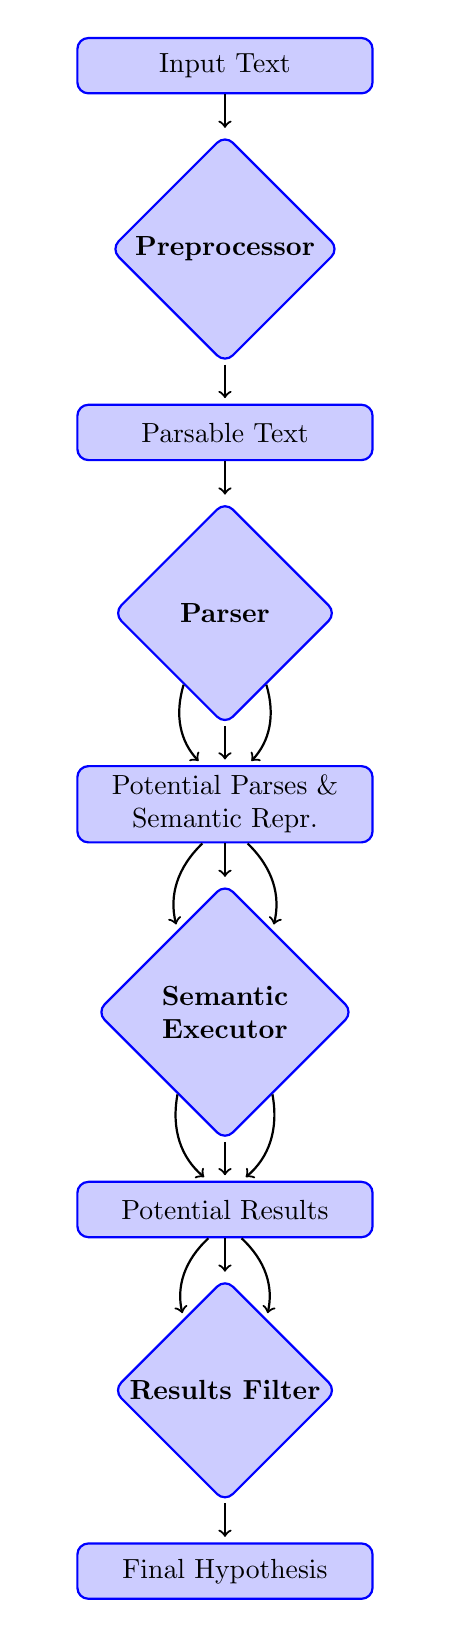
\begin{tikzpicture} [
            auto,
            decision/.style = { diamond, draw=blue, thick, fill=blue!20,
                                text width=7em, text badly centered,
                                inner sep=1pt, rounded corners },
            block/.style    = { rectangle, draw=blue, thick,
                                fill=blue!20, text width=10em, text centered,
                                rounded corners, minimum height=2em },
            line/.style     = { draw, thick, ->, shorten >=2pt },
          ]
          \matrix [column sep=5mm, row sep=5mm] {
            & \node (in1) [block, ] {Input Text}; & \\
            & \node (pro1) [decision] {\textbf{Preprocessor}}; & \\
            & \node (in2) [block] {Parsable Text}; & \\
            & \node (pro2) [decision] {\textbf{Parser}}; & \\
            & \node (in3) [block] {Potential Parses \& \\ Semantic Repr.}; & \\
            & \node (pro3) [decision] {\textbf{Semantic Executor}}; & \\
            & \node (in4) [block] {Potential Results}; & \\
            & \node (pro4) [decision] {\textbf{Results Filter}}; & \\
            & \node (dec1) [block] {Final Hypothesis}; & \\
          };

            \draw [line] (in1) edge (pro1);
            \draw [line] (pro1) edge (in2);
            \draw [line] (in2) edge (pro2);
            \draw [line] (pro2) edge (in3);
            \draw [line, bend right] (pro2) edge (in3);
            \draw [line, bend left] (pro2) edge (in3);
            \draw [line] (in3) edge (pro3);
            \draw [line, bend right] (in3) edge (pro3);
            \draw [line, bend left] (in3) edge (pro3);
            \draw [line] (pro3) edge (in4);
            \draw [line, bend right] (pro3) edge (in4);
            \draw [line, bend left] (pro3) edge (in4);
            \draw [line] (in4) edge (pro4);
            \draw [line, bend right] (in4) edge (pro4);
            \draw [line, bend left] (in4) edge (pro4);
            \draw [line] (pro4) edge (dec1);
        \end{tikzpicture}
        \caption{Flow of data through our semantic parsing and solving engine.}
        \label{fig:flowchart}
    \end{minipage}
\end{figure}

\subsection{Preprocessor}

Before entering the semantic parser, all input to our system passes through a preprocessor first. There are several steps to the preprocessor that improve the semantic parser's ability to handle a broad range of text. Adding these steps dramatically improved our system's overall performance.

First, we apply a simple regular expression engine to the text to make all tokens lowercase and to split punctuation from words and into their own tokens. This step significantly cuts down on the number of rules required (for example, because ``number'' will be treated the same as ``Number'').

In the preprocessor, we take an important step to disambiguate some locally-unresolvable coreference issues. A semantic parser steps through tokens and builds up a semantic representation in a tree-like fashion. Consider the sentence: ``Two numbers have a sum of ten and their product is twenty-four''. The correct series of equations to extract is ``x+y = 10'' and ``x*y = 24'' (the solution is 4 and 6). However, during the semantic parser's execution, by the time it reaches the subphrase ``their product,'' it has already forgotten that there are two numbers in the first equation. Locally, it has no way to conclude that x*y=24 is more correct than x*y*z = 24, or is better than an equation codifying that the product of fifteen numbers is 24. To solve this fairly frequent type of scenario, we preprocess the text and use basic heuristics to identify how many numbers are in the solution set. We can then replace the text ``their product'' with new text ``their\_3 product''. We can then have rules like ``their\_N'' for any generic N. We preprocess prefix words like ``their, whose'' and different operations like ``product, sum, average''.


\subsection{Parser}

We use Sippycup as our semantic parser. While not an ``industrial-strength'' semantic parser, we found its Pythonic interface and our previous experience with the library gave it a significant advantage over other systems like SEMPRE, which have more complex capabilities, but much higher learning curves. As witnessed through SigmaDolphin, semantic parsing requires a large number of rules to get off the ground and start producing results. We created 6,204 semi-automatically generated rules to parse the questions. At the start, many of the rules dealt with converting integers to strings and vice-versa. Our system had to understand a question regardless of how the integers were stated. For example, the two questions below have identical semantics and are just represented differently in text.

\begin{center}
    \textit{``The sum of \underline{two} numbers is \underline{seventy-two}''\\
    ``The sum of \underline{2} numbers is \underline{72}.''}
\end{center}

Building off the integer rules, we added many rules related to junk words, like ``an'' or ``the.'' Our flexible set of junk rules allowed us to treat small variations in sentence structure as identical and thus resulting in the same semantic representations. While these types of rules are simple, they are integral to a successful parser and helped us build up the rest of our rules.

We are particularly proud of the way we handled terms like ``the largest number'' in examples such as ``the smallest plus the largest equals 25.'' In this situation, the semantic parser can't know if ``the largest'' is the second, third, fourth, or five-hundredth variable in this equation. Throughout the examples in this paper, we've used common variable names like x and y, but in the parser, we use variables called ``v0'' up through ``vN.'' When parsing something like ``the largest'' or ``the second largest'' we can pretend as though there is a variable called ``v-1'' and ``v-2''. At the end, during semantic evaluation, we can replace ``v-1'' with whatever ``N-1'' is for this particular series of equations. This is an example of one place where we correct incomplete local data with the correct, globally consistent semantic meaning later on.

\subsection{Semantic Executor}
Once our semantic parser generates a semantic representation of a question, the next step is to take that representation (a s-expression) and turn it into a string equation that can be fed into SymPy. As mentioned above, the recursive structure of s-expressions lends itself to well to this task. Surprisingly, we encountered a lot of difficulty at this stage. For example, if we look at a few example s-expressions in Table ~\ref{tab:s-expr-examples}, it quickly becomes apparent that we need to distinguish between unary (abs(), \string^2, \string^3) and binary (+, -, *, and /) relations as well as be flexible with the number of possible operands for a given operator and honoring the correct order of operations.

\begin{table*}[t]
    \centering
    \begin{tabular}{|c|c|}
        \hline
        \textbf{S-expression} & \textbf{String Equation} \\ \hline
        \texttt{(= x (+ 5 y)) } & \texttt{ x = 5 + y} \\ \hline
        \texttt{(= x (\string^ 2 5)) } & \texttt{ x = 5\string^2 } \\ \hline
        \texttt{(= x (+ 10 5 (* 5 y)))} & \texttt{ x = 10 + 5 + 5*y} \\ \hline
        \texttt{(= x (* (10 (+ 5 y))))} & \texttt{ X = (5 + y) * 10} \\ \hline
    \end{tabular}
    \caption{Example s-expressions.}
    \label{tab:s-expr-examples}
\end{table*}

\begin{table*}[t]
    \centering
    \begin{tabularx}{\linewidth}{|X|X|X|}
        \hline
        \textbf{Question} & \textbf{Our Parse} & \textbf{Correct Parse} \\ \hline
        The difference of the reciprocals of two consecutive integers is 1/72. Find the smaller of the two integers
        &
        \small {\texttt{(= (/ 1 72) (- ((\string^(-1) y) \newline \hspace*{1em} (\string^(-1), x))) } }\newline
        \small {\texttt{(= x x) } }\newline
        \small {\texttt{(= y (+ x 1))}}
        &
        \small {\texttt{(= (/ 1 72) (- ((\string^(-1) x) \newline \hspace*{1em} (\string^(-1), y))) } }\newline
        \small {\texttt{(= x x) } }\newline
        \small {\texttt{(= y (+ x 1))}}
        \\
        % empty
        &
        \small {\texttt{(1/y)-(1/x) = (1/72) } }\newline
        \small {\texttt{y = x + 1 } }\newline
        \small {\texttt{No real answer!}}
        &
        \small {\texttt{(1/x)-(1/y) = (1/72) } }\newline
        \small {\texttt{x = x, y = x + 1 } }\newline
        \small {\texttt{x = -9 or x = 8} }
        \\
        \hline
        The difference of the squares of two positive consecutive even integers is 44. Find the integers
        &
        \small{ \texttt{(= (- ((\string^2 y), (\string^2 y))), \newline \hspace*{1em} 44) }} \newline
        \small{ \texttt{(= x (* 2 k) }} \newline
        \small{ \texttt{(= y (+ (* 2 k) 2)) }}
        &
        \textbf{We parsed this problem \newline correctly}
        \\
        % empty
        &
        \small{ \texttt{(y\string^2)-(x\string^2) = 44}} \newline
        \small{ \texttt{x = 2*k, y = 2*k + 2}} \newline
        \small{ \texttt{k = 5, x = 10, y = 12}}
        &
        % empty
        \\
        \hline
    \end{tabularx}
    \caption{Worked examples of input text, s-expressions, and semantic equations.}
    \label{tab:full-parsing}
\end{table*}

Table ~\ref{tab:full-parsing} highlights the difficulties with some of the more complicated parses. For instance, imagine we are trying to create a general rule tailored around the word ``difference''. In most cases, if we see the sentence ``the difference of x and y is 72'', the translation can be the equation: (y - x) = 72. We can see this logic working in the second example above. The problem is that this won't always generate real answers. One possible solution is to generate a lot more parses, interpreting the same question in multiple ways. For example, we could choose to parse ``the difference of x and y is 72'' as both (y - x) = 72 and (x -y) = 72 or just as abs(x - y) = 72. Yet, this ``solution'' only pushes back the problem to the result picker phase and can add wrong parses to the ``difference'' problems. We still need the additional context of the sentence to determine which answer we need. The second example points us in the right direction with the ``two positive consecutive even integers''. The first example doesn't give us any constraints and would accept both positive and negative numbers. We, however, kept parsing ``difference'' questions as (x - y) due to the fact that this largely gave us the right answer and  did not require even more processing of the question. It should be noted that tackling these types of semantic particulars is important for a state of the art parser and would definitely be a good avenue for future work. After the string equation is formed from the parse, it is relatively simply to feed in the result into SymPy's solver method and get the result or results out.

\subsection{Result Filter}
For a given question, our set of grammar rules can come up with upwards of 128 different parses. Our executor then takes those parses, tries to turn them into equations, and solves them using SymPy. After this step, we are often left with multiple answers for the question. In order to choose a right answer, we follow a couple of guidelines. First, we need to weed out the non-real answers. Any answers in terms of the complex number i or variables still present are removed from the set of answers. These types of answers occur because that parse was incorrect -- since we know that non-real numbers and underdefined systems are not part of the domain's solution space, we can easily reject those parses as spurious. Next, we sort the answers by the number of occurrences in the answer set. If there is a most popular answer, we choose that one. If not, we continue to filter the answers further down to the set of most popular. Afterwards, we check if the answers are positive or negative. If the question text doesn't contain a negative constraint word like ``negative'' or ``nonpositive'', we remove all negative answers from our set of answers. Lastly, if we still have more than one answer left, we randomly pick the an answer out of the set.

Although this methodology is crude and simple, it does remarkably well within this domain, helping us get an accuracy of 78.3\% on questions that we found parses for. The questions we got wrong (21.7\%) were a mixture of incorrect parses or random guesses where we had the right answer, but we guessed the wrong one.

\section{Discussion}
The system presented here is an excellent example of applying semantic parsing to a complex and real-world domain. It represents both the positive aspects of using semantic parsing in addition to the challenges that are inherent to the tool and fundamentally limit its practical use. We explore both these facets in detail. Semantic parsing is quick to get started, and once the first input is parsed, huge swaths of the new examples in the corpus can be properly parsed each time a single additional rule is added. This ability to get moving quickly with no training data is a boon to researchers and professional users of NLP technology. We experienced this ourselves, as the first 25\% of the corpus was parsed with only a handful of clever and basic rules.

Out of the 6240 rules, a full 89\% are just the positive and negative numbers between -1000 and 1000 written out in numerals and in words (in a few different forms). Another 404 are in the so-called \texttt{\$Junk} category -- a catchall for any word in the vocabulary that we deem as unimportant. These words usually show up in the preamble or epilogue of a question: ``Two numbers sum to six and have a product of eight. \textit{Find the numbers}''. Although these rules make up the vast, vast majority of the total grammar rules in SippyCup, they represent an incredibly small fraction of developer time. Included in this report as Figure \ref{fig:chart} is a graph of which parsing tokens appear the most often on the left-hand side.  The graph shows the classic ``long tail'' of rules -- many rules appear only once or twice on the right hand side (although this is largely an artifact of SippyCup, which prevents nonterminals and terminals from both being on the right of one grammar rule). The top two classes (\texttt{\$Num} and \texttt{\$Junk} are excluded, since they are both more than an order of magnitude larger than the next class). The most common rules are those dealing with operators between two operands, for example, different terms that could be substituted in the phrase ``x \textit{plus} y''. A full list of the rules is, obviously, included with our code.

\begin{figure*}[t]
    \centering
    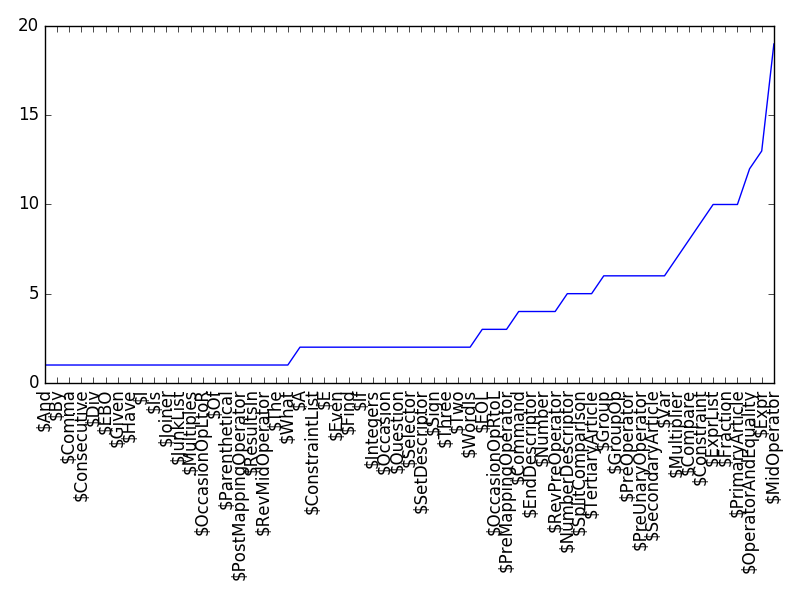
\includegraphics[width=0.85\textwidth]{rules-bottom.png}
    \caption{The number of rules with the given left-hand side. The top two are ommitted, as they were not hand-written.}
    \label{fig:chart}
\end{figure*}

Reaching our parse percentage of 48.3\% required 225 handwritten rules specific to this domain, each one invented by manually inspecting development set questions to come up with clever ways to generically capture specific semantic meaning. While 225 rules seems like a small amount, this required significant investment. As more semantic parsing rules are written and rule authors take advantage of all the ``quick wins,'' the marginal parsing value from each rule is low. Adding another 225 handwritten rules would likely struggle to parse an additional significant portion of the dataset.
Semantic parsing breaks when a large portion of text is unconventional or breaks from the domain's usual pattern substantially. The system described here performs admirably when tasked with solving ``regular''-sounding algebra word problems. However, no matter how many rules, semantic parsing in its current form will never be able provide a parse to ever example in its domain -- natural language is simply too complex to be constrained to the same types of context-free grammar rules used to describe compiler operations.


\section{Conclusion}
Our implementation of a SippyCup-based semantic parsing solution for solving simple word problems provides similar results to those of the current state of the art and reinforces the notion that while initially promising, semantic parsing does not lend itself to creating a robust solution system with a highly variable domain. Our recall percentage and accuracy is lower than that of SigmaDolphin, currently the most sophisticated semantic parsing solution to this problem. However, we have only 65\% the number of rules that SigmaDolphin implements, which indicates that after the initial rules are completed, the marginal cost for each additional successful parse is quite high.

Given a correct parse, the accuracy demonstrated by our system and SigmaDolphin represent the fact that semantic parsing is still extremely accurate. Significant future work should be invested into systems that combine semantic parsing with other, more automatic or statistical methods of NLP that will hopefully result in a hybrid combination of semantic parsing's accuracy and statistical methods ability to generalize across a varied domain.

\section{Code}
The code for this project is available at \url{https://github.com/sloanesturz/cs224u-final-project}.

\newpage
% include your own bib file like this:
%\bibliographystyle{acl}
%\bibliography{acl2014}
%
\begin{thebibliography}{}
% %  Example
\bibitem[\protect\citename{Shi et al.} 2015]{Shi:15}
Shuming Shi, Yuehui Wang, Chin-Yew Lin, Xiaojiang Liu, and Yong Rui.
\newblock 2015
\newblock {\em Automatically Solving Number Word Problems by Semantic Parsing and Reasoning}. Link: http://aclweb.org/anthology/D15-1135

\bibitem[\protect\citename{Kushman et al.} 2014]{Kushman:14}
Nate Kushman, Yoav Artzi, Luke Zettlemoyez, and Regina Barzilay.
\newblock 2014
\newblock {\em Learning to Automatically Solve Algebra Word Problems}. Link: http://yoavartzi.com/pub/kazb-acl.2014.pdf

\bibitem[\protect\citename{Morton et al.} 2012]{Morton:12}
Kyle Morton and Yanzhen Qu.
\newblock 2012
\newblock {\em A Novel Framework for Math Word Problem Solving}. Link: http://www.ijiet.org/papers/240-T0031.pdf
\end{thebibliography}

\end{document}
